% !TeX spellcheck = ru_RU
\documentclass[a4paper,12pt]{extarticle}
\usepackage[utf8x]{inputenc}
\usepackage[T1,T2A]{fontenc}
\usepackage[russian]{babel}
\usepackage{hyperref}
\usepackage{indentfirst}
\usepackage{listings}
\usepackage{color}
\usepackage{here}
\usepackage{array}
\usepackage{multirow}
\usepackage{graphicx}

\usepackage{caption}
\renewcommand{\lstlistingname}{Программа} % заголовок листингов кода

\bibliographystyle{ugost2008ls}

\usepackage{listings}
\lstset{ %
extendedchars=\true,
keepspaces=true,
language=C,						% choose the language of the code
basicstyle=\footnotesize,		% the size of the fonts that are used for the code
numbers=left,					% where to put the line-numbers
numberstyle=\footnotesize,		% the size of the fonts that are used for the line-numbers
stepnumber=1,					% the step between two line-numbers. If it is 1 each line will be numbered
numbersep=5pt,					% how far the line-numbers are from the code
backgroundcolor=\color{white},	% choose the background color. You must add \usepackage{color}
showspaces=false				% show spaces adding particular underscores
showstringspaces=false,			% underline spaces within strings
showtabs=false,					% show tabs within strings adding particular underscores
frame=single,           		% adds a frame around the code
tabsize=2,						% sets default tabsize to 2 spaces
captionpos=t,					% sets the caption-position to top
breaklines=true,				% sets automatic line breaking
breakatwhitespace=false,		% sets if automatic breaks should only happen at whitespace
escapeinside={\%*}{*)},			% if you want to add a comment within your code
postbreak=\raisebox{0ex}[0ex][0ex]{\ensuremath{\color{red}\hookrightarrow\space}},
texcl=true,
inputpath=listings,                     % директория с листингами
}

\usepackage[left=2cm,right=2cm,
top=2cm,bottom=2cm,bindingoffset=0cm]{geometry}

%% Нумерация картинок по секциям
\usepackage{chngcntr}
\counterwithin{figure}{section}
\counterwithin{table}{section}

%%Точки нумерации заголовков
\usepackage{titlesec}
\titlelabel{\thetitle.\quad}
\usepackage[dotinlabels]{titletoc}

%% Оформления подписи рисунка
\addto\captionsrussian{\renewcommand{\figurename}{Рисунок}}
\captionsetup[figure]{labelsep = period}

%% Подпись таблицы
\DeclareCaptionFormat{hfillstart}{\hfill#1#2#3\par}
\captionsetup[table]{format=hfillstart,labelsep=newline,justification=centering,skip=-10pt,textfont=bf}

%% Путь к каталогу с рисунками
\graphicspath{{fig/}}

%% Внесение titlepage в учёт счётчика страниц
\makeatletter
\renewenvironment{titlepage} {
 \thispagestyle{empty}
}
\makeatother

\usepackage{minted}

\begin{document}	% начало документа

% Титульная страница
\begin{titlepage}	% начало титульной страницы

	\begin{center}		% выравнивание по центру

		\large Санкт-Петербургский Политехнический Университет Петра Великого\\
		\large Институт компьютерных наук и технологий \\
		\large Кафедра компьютерных систем и программных технологий\\[6cm]
		% название института, затем отступ 6см
		
		\huge Базы данных\\[0.5cm] % название работы, затем отступ 0,5см
		\large Отчет по лабораторной работе №1\\[0.1cm]
		\large Разработка структуры БД\\[5cm]

	\end{center}


	\begin{flushright} % выравнивание по правому краю
		\begin{minipage}{0.25\textwidth} % врезка в половину ширины текста
			\begin{flushleft} % выровнять её содержимое по левому краю

				\large\textbf{Работу выполнил:}\\
				\large Графов Д.И.\\
				\large {Группа:} 33531/2\\
				
				\large \textbf{Преподаватель:}\\
				\large Мяснов А.В.

			\end{flushleft}
		\end{minipage}
	\end{flushright}
	
	\vfill % заполнить всё доступное ниже пространство

	\begin{center}
	\large Санкт-Петербург\\
	\large \the\year % вывести дату
	\end{center} % закончить выравнивание по центру

\thispagestyle{empty} % не нумеровать страницу
\end{titlepage} % конец титульной страницы

\vfill % заполнить всё доступное ниже пространство


\newpage
\setcounter{page}{2}
% Содержание
% Содержание
\renewcommand\contentsname{\centerline{Содержание}}
\tableofcontents
\newpage



\section{Цель работы}
Познакомиться с основами проектирования схемы БД, способами организации данных в SQL-БД.

\section{Программа работы}
	\begin {enumerate}
	\item Создание проекта для работы в GitLab.
	\item Выбор задания (предметной области), описание набора данных и требований к хранимым данным в свободном формате в wiki своего проекта в GitLab.
	\item Формирование в свободном формате (предпочтительно в виде графической схемы) cхемы БД, соответствующей заданию. Должно получиться не менее 7 таблиц.
	\item Согласование с преподавателем схемы БД. Обоснование принятых решений и соответствия требованиям выбранного задания. 
	\item Выкладывание схемы БД в свой проект в GitLab.
	\item Демонстрация результатов преподавателю.
	\end {enumerate}

\section{Теоретическая информация}

\begin {itemize}
\item \textbf{Первичный ключ (primary key)} представляет собой один из примеров уникальных индексов и применяется для уникальной идентификации записей таблицы. Никакие из двух записей таблицы не могут иметь одинаковых значений первичного ключа. Первичный ключ обычно сокращенно обозначают как PK (primary key).

\item \textbf{Внешний ключ} — это столбец или комбинация столбцов, значения которых соответствуют Первичному ключу в другой таблице. Связь между двумя таблицами задается через соответствие Первичного ключа в одной из таблиц внешнему ключу во второй.
\end {itemize}

\section{Выполнение работы}


\subsection{Выбор предметной области}

В качестве предметной области был выбран каталог баров. База данных хранит перечень баров, а также еды и напитков.

\subsection{Описание таблиц}
\begin{itemize}
	\item components - ингредиенты для напитков. Имеет поля, в которых указывается название и процент алкоголя.
	\item drinks - напитки. Поля: название, рейтинг, объём, процент алкоголя, средняя цена, тип напитка.
	\item places - заведения. Поля: название, адрес, рейтинг, средний счёт.
	\item food - еда. Поля: название, рейтинг, объём, средняя цена.
	\item discounts - скидки. Поля: заведение(внешний ключ), тип напитка, процент скидки, описание, день недели, время начала, время конца.
	\item supplies\_drinks - поставки напитков. Поля: заведение(внешний ключ), идентефикатор напитка, количество, цена за еденицу, дата.
	\item supplies\_food -поставки еды. Поля: заведение(внешний ключ), идентефикатор еды, количество, цена за еденицу, дата.
	\item Вспомогательные: 
		\begin {itemize}
		\item components\_drinks
		\item places\_drinks
		\item places\_food
	\end {itemize}
\end{itemize}


\subsection{Структура базы данных}

\begin{figure}[H]
	\begin{center}
		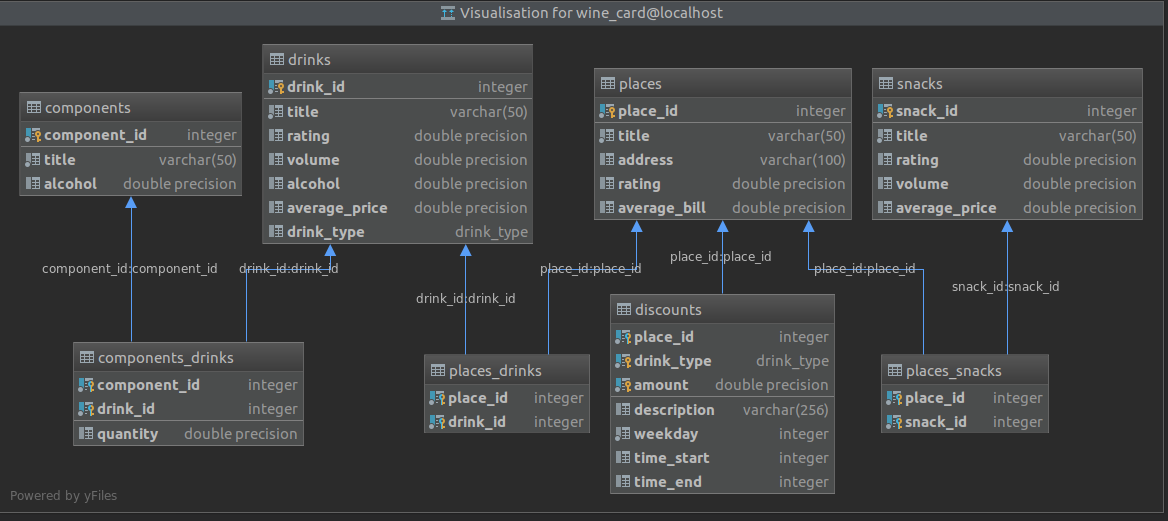
\includegraphics[scale=0.3]{../../structure.png}
		\caption{Структура базы данных} 
		\label{pic:struct} % название для ссылок внутри кода
	\end{center}
\end{figure}

\section{Выводы}

В ходе выполнения данной работы была спроектирована и согласована с преподавателем база данных, содержащая перечень баров, а также еды и напитков. Также были изучены такие понятия, как Primary Key (PK) и Foreign Key (FK).

\end{document}

